\documentclass[11pt]{amsart}

\usepackage{amsthm}
	\newtheorem*{theorem}{Theorem}
\usepackage{cleveref}

\usepackage[margin=1in]{geometry}

\usepackage{tikz} 
	\usetikzlibrary{patterns}
	\usetikzlibrary{cd}
	
\usepackage{xcolor}
	\definecolor{umaroon}{RGB}{122,0,25}

\title{An example illustrating the Siefert-van Kampen theorem}
\author{Trevor K. Karn}
\address{206 Church Street SE, Minneapolis, USA}
%\curraddr{}
\email{karnx018@umn.edu}
\thanks{I would like to thank Tomas Ba\~nuelos, Casey Garner, and Jacob Hegna for helpful conversations during the writing of this note.}

\begin{document}

\maketitle

\section{Introduction}

When I first read Hatcher's classic text \textit{Algebraic Topology} I did not understand the Siefert-van Kampen theorem at all. When I took MATH 8301 - Manifolds and Topology at the University of Minnesota, I understood it a little better, but still struggled. Then I started to study for the Preliminary exam in topology, and so I worked through this example, and it helped me to understand it better. So I thought I would write up the example and some background to say what I found confusing in hopes that it might help someone else understand the theorem better. On the other hand, maybe I'm just a big dummy and others find this theorem less confusing than I did. 
At any rate, enjoy!

\section{Introducing the example}

The topological space we consider can be though of as the union of two partially-overlapping circles $A$ and $B$, with a few regions punched out. We'll put a basepoint $x_0$ in the intersection. We will also punch out two regions from the interior of the intersection $A \cap B$, and we will also punch out a region from the interior of $A-B$ and $B-A$. We sketch this in \Cref{fig:Xnoloops}. 
Anyone who is familiar with the fundamental group will immediately recognize that, since there are four holes punched out, then $\pi_1(X) = \langle x_1, x_2, x_3, x_4 \rangle$ is the free group on four letters. With this example, it is not so hard to just compute the fundamental group $\pi_1(X)$. On the other hand thinking of $A$ and $B$ as a cover of $X$, we can use this example to understand how $\pi_1(A)$ and $\pi_1(B)$ are related to $\pi_1(X)$. 

\begin{center}
\begin{figure}[h]
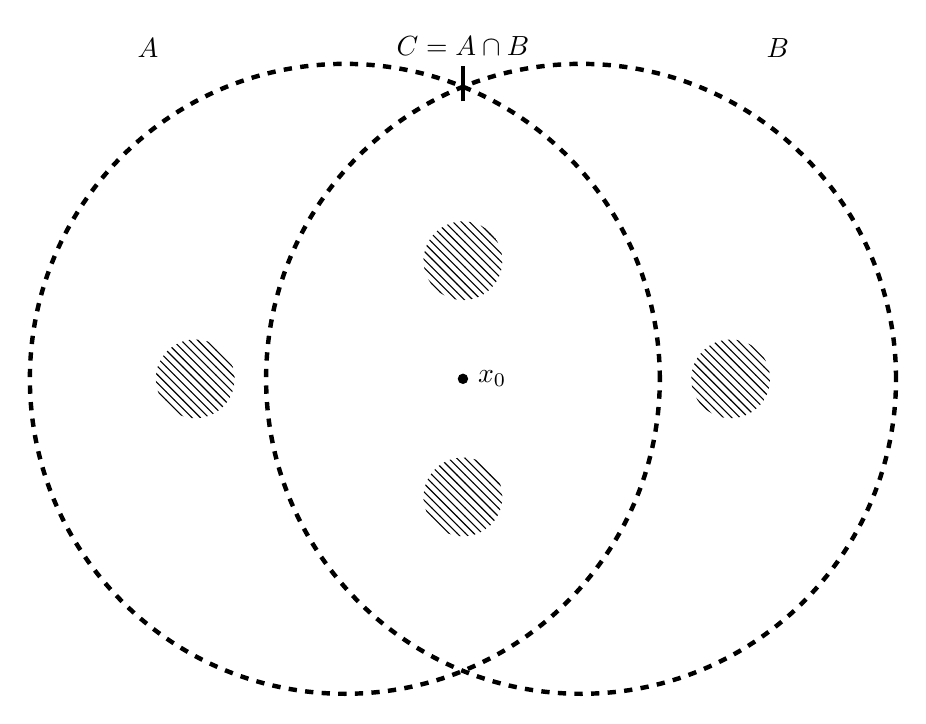
\begin{tikzpicture}
	\draw[ultra thick, dashed] (-1.5,0) circle (4cm);
	\draw[ultra thick, dashed] (1.5,0) circle (4cm);
	\draw[pattern = north west lines, draw=none] (0,1.5) circle (0.5 cm);
	\draw[pattern = north west lines, draw=none] (0,-1.5) circle (0.5 cm);
	\draw[pattern = north west lines, draw=none] (3.4,0) circle (0.5 cm);
	\draw[pattern = north west lines, draw=none] (-3.4,0) circle (0.5 cm);
	
%	\draw[thick, color=blue, densely dotted] (0,0) .. controls (-3,3)  and (3,3) ..  (0,0);
%	\draw[thick, densely dotted, color=umaroon] (0,0) .. controls (-3,-3)  and (3,-3) ..  (0,0);
%	\draw[thick, dashed] (0,0) .. controls (7,5) and (7,-5) .. (0,0);
%	\draw[thick] (0,0) .. controls (-7,5) and (-7,-5) .. (0,0);
%	
%	\draw[thick, color=blue] (0,0) .. controls (-6,5) and (5,4)  .. (0,0);
%	\draw[thick, color=blue, dashed] (0,0) .. controls (6,5) and (-5,4)  .. (0,0);
%	
%	\draw[thick, color=umaroon] (0,0) .. controls (-6,-5) and (5,-4)  .. (0,0);
%	\draw[thick, color=umaroon, dashed] (0,0) .. controls (6,-5) and (-5,-4)  .. (0,0);
%	
	\node[fill=black, circle, scale = 0.4, label=right:$x_0$] (0,0) {};
%	
%	\node[] at (-3.4,1.7) {$a_3$};
%	\node[] at (3.4,1.7) {$b_3$};
%	
%	\node[] at (-2.2,2.9) {$a_1$};
%	\node[] at (2.2,2.9) {$b_1$};
%	
%	\node[] at (-2.2,-2.9) {$a_2$};
%	\node[] at (2.2,-2.9) {$b_2$};
%	
%	\node[] at (0,2.5) {$c_1$};
%	\node[] at (0,-2.5) {$c_2$};
	
	\node[] at (-4,4.2) {$A$};
	\node[] at (4,4.2) {$B$};
	
	\node[pin={[pin edge={ultra thick,black}]$C=A\cap B$}] at (0,3.4) {};
	
\end{tikzpicture}
\caption{The main topological space $X = A \cup B$ we consider}\label{fig:Xnoloops}
\end{figure}
\end{center}

We can compute $\pi_1(A)$ quite easily by observing there are three homotopy classes of loops in $A$, so $\pi_1(A) = \langle a_1, a_2, a_3 \rangle$, where we identify the loops drawn in \Cref{fig:A} with their representatives in $\pi_1(A)$. In particular, I took care to draw $a_1$ and $a_2$ so that they are \textit{not} contained in $C$. Of course, they are homotopic in $A$ (and in $X$) to loops which do lie in $C$, but I want to make the distinction between loops in $A$ and loops in $C$. Since $a_1, a_2$ are not contained in $C$, there is no risk of confusing them for loops in $C$. 

\begin{center}
\begin{figure}[t]
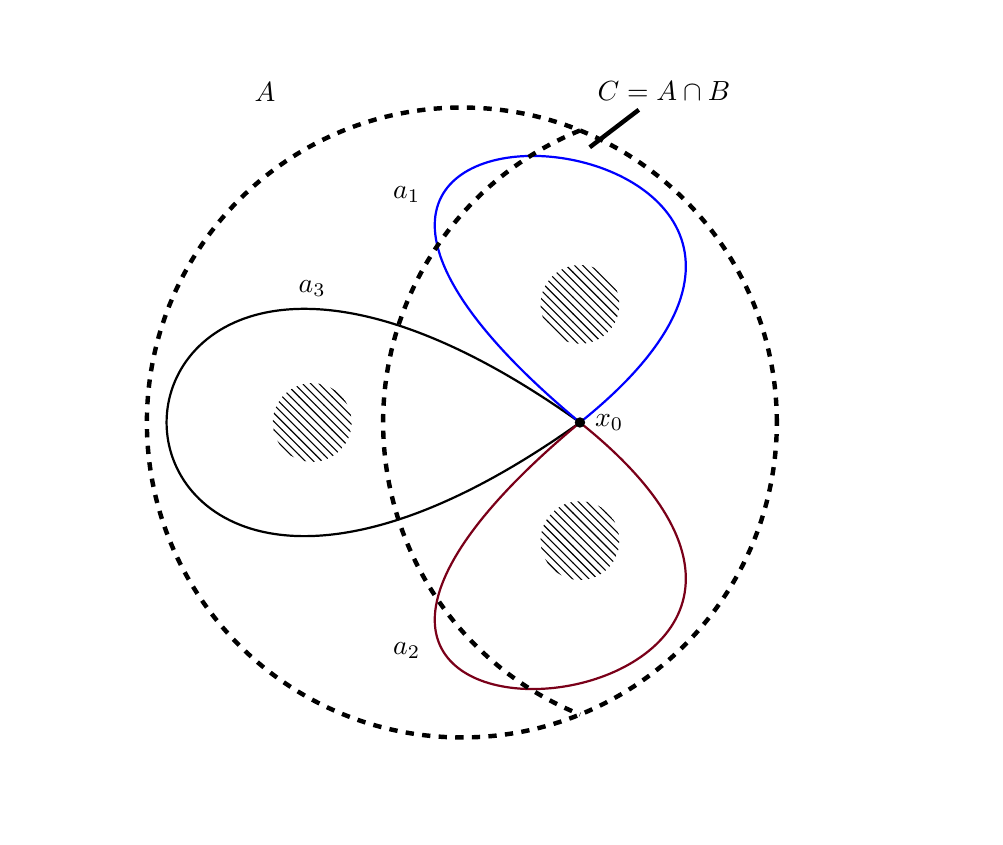
\begin{tikzpicture}
	\draw[ultra thick, dashed] (-1.5,0) circle (4cm);
	%\draw[ultra thick, dashed] (1.5,0) circle (4cm);
	\draw[pattern = north west lines, draw=none] (0,1.5) circle (0.5 cm);
	\draw[pattern = north west lines, draw=none] (0,-1.5) circle (0.5 cm);
	%\draw[pattern = north west lines, draw=none] (3.4,0) circle (0.5 cm);
	\draw[pattern = north west lines, draw=none] (-3.4,0) circle (0.5 cm);
	
	%\draw[thick, color=blue, densely dotted] (0,0) .. controls (-3,3)  and (3,3) ..  (0,0);
	%\draw[thick, densely dotted, color=umaroon] (0,0) .. controls (-3,-3)  and (3,-3) ..  (0,0);
	%\draw[thick, dashed] (0,0) .. controls (7,5) and (7,-5) .. (0,0);
	\draw[thick] (0,0) .. controls (-7,5) and (-7,-5) .. (0,0);
	
	\draw[thick, color=blue] (0,0) .. controls (-6,5) and (5,4)  .. (0,0);
	%\draw[thick, color=blue, dashed] (0,0) .. controls (6,5) and (-5,4)  .. (0,0);
	
	\draw[thick, color=umaroon] (0,0) .. controls (-6,-5) and (5,-4)  .. (0,0);
	%\draw[thick, color=umaroon, dashed] (0,0) .. controls (6,-5) and (-5,-4)  .. (0,0);
	
	\node[fill=black, circle, scale = 0.4, label=right:$x_0$] (0,0) {};
	
	\node[] at (-3.4,1.7) {$a_3$};
	%\node[] at (3.4,1.7) {$b_3$};
	
	\node[] at (-2.2,2.9) {$a_1$};
	%\node[] at (2.2,2.9) {$b_1$};
	
	\node[] at (-2.2,-2.9) {$a_2$};
	%\node[] at (2.2,-2.9) {$b_2$};
	
	%\node[] at (0,2.5) {$c_1$};
	%\node[] at (0,-2.5) {$c_2$};
	
	\node[] at (-4,4.2) {$A$};
	%\node[] at (4,4.2) {$B$};
	
	\node[pin={[pin edge={ultra thick,black}]80:$C=A\cap B$}] at (0,3.4) {};
	\draw [ultra thick,domain=112:248,samples=400,dashed] plot ({4*cos(\x)+1.5}, {4*sin(\x)});
	
\end{tikzpicture}
\caption{Computing the fundamental group of $A$}\label{fig:A}
\end{figure}
\end{center}

We can reflect everything in this situation symmetrically about the middle to find loops $b_1, b_2, b_3$ in $B$ such that - in $X$ - we have $b_1 \sim a_1$ and $b_2 \sim a_2$, but then $b_3$ loops around the punched out region which is contained in $B-A$. From this we see by symmetry that $\pi_1(B) = \langle b_1, b_2, b_3 \rangle$.

The final piece of the puzzle which we'll focus on is the space $C = A \cap B$.
There are two distinct (nonidentity) homotopy classes of loops, shown in figure \Cref{fig:C}. Thus we see that $\pi_1(C) = \langle c_1, c_2 \rangle$. 

\begin{center}
\begin{figure}[h]
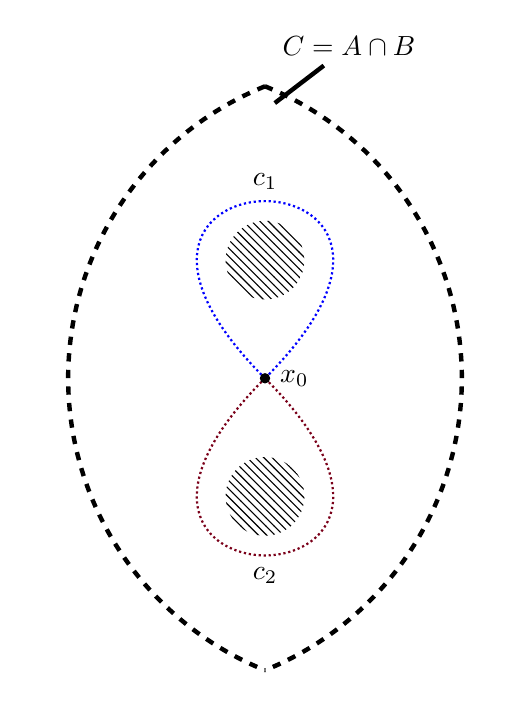
\begin{tikzpicture}
	%\draw[ultra thick, dashed] (-1.5,0) circle (4cm);
	%\draw[ultra thick, dashed] (1.5,0) circle (4cm);
	\draw[pattern = north west lines, draw=none] (0,1.5) circle (0.5 cm);
	\draw[pattern = north west lines, draw=none] (0,-1.5) circle (0.5 cm);
	%\draw[pattern = north west lines, draw=none] (3.4,0) circle (0.5 cm);
	%\draw[pattern = north west lines, draw=none] (-3.4,0) circle (0.5 cm);
	
	\draw[thick, color=blue, densely dotted] (0,0) .. controls (-3,3)  and (3,3) ..  (0,0);
	\draw[thick, densely dotted, color=umaroon] (0,0) .. controls (-3,-3)  and (3,-3) ..  (0,0);
	%\draw[thick, dashed] (0,0) .. controls (7,5) and (7,-5) .. (0,0);
	%\draw[thick] (0,0) .. controls (-7,5) and (-7,-5) .. (0,0);
	
	%\draw[thick, color=blue] (0,0) .. controls (-6,5) and (5,4)  .. (0,0);
	%\draw[thick, color=blue, dashed] (0,0) .. controls (6,5) and (-5,4)  .. (0,0);
	
	%\draw[thick, color=umaroon] (0,0) .. controls (-6,-5) and (5,-4)  .. (0,0);
	%\draw[thick, color=umaroon, dashed] (0,0) .. controls (6,-5) and (-5,-4)  .. (0,0);
	
	\node[fill=black, circle, scale = 0.4, label=right:$x_0$] (0,0) {};
	
	%\node[] at (-3.4,1.7) {$a_3$};
	%\node[] at (3.4,1.7) {$b_3$};
	
	%\node[] at (-2.2,2.9) {$a_1$};
	%\node[] at (2.2,2.9) {$b_1$};
	
	%\node[] at (-2.2,-2.9) {$a_2$};
	%\node[] at (2.2,-2.9) {$b_2$};
	
	\node[] at (0,2.5) {$c_1$};
	\node[] at (0,-2.5) {$c_2$};
	
	%\node[] at (-4,4.2) {$A$};
	%\node[] at (4,4.2) {$B$};
	
	\node[pin={[pin edge={ultra thick,black}]80:$C=A\cap B$}] at (0,3.4) {};
	\draw [ultra thick,domain=112:248,samples=400,dashed] plot ({4*cos(\x)+1.5}, {4*sin(\x)});
	\draw [ultra thick,domain=428:292,samples=400,dashed] plot ({4*cos(\x)-1.5}, {4*sin(\x)});
	
\end{tikzpicture}
\caption{Computing the fundamental group of $C$}\label{fig:C}
\end{figure}
\end{center}

\section{Statement of the theorem}

There are a few different ways to think of the statement of the theorem (for example in terms of pushouts and pull backs), but for the sake of this example we'll look at the way that Hatcher explains it. 
First, Hatcher defines inclusion map $i_{\alpha \beta}: \pi_1(A_\alpha \cap A_\beta) \rightarrow \pi_1(A_\alpha)$ where you take a loop in $A_\alpha \cap A_\beta$ and consider it as a loop in $A_\alpha$. Then he extends the inclusion map $j_\alpha: \pi_1(A_\alpha) \rightarrow \pi_1(X)$ to $\Phi: *_\alpha \pi_1(A_\alpha) \rightarrow \pi_1(X)$. The point of this map is to think of loops in $\pi_1(A_\alpha)$ as loops in $X$, but doing it for every loop in every component $A_\alpha$
The exact statement in Hatcher is given below.

\begin{theorem}[Siefert-van Kampen]
If $X$ is the union of path-connected open sets $A_\alpha$ each containing the basepoint $x_0$, and if each intersection $A_\alpha \cap A_\beta$ is path connected, then the homomorphism ${\Phi : *_\alpha \pi_1(A_\alpha) \rightarrow \pi_1(X)}$ is surjective. If, in addition, each intersection $A_\alpha \cap A_\beta \cap A_\gamma$ is path connected, then the kernel of $\Phi$ is the normal subgroup $N$ generated by all elements of the form $i_{\alpha\beta} (w) i_{\beta\alpha}(w)^{-1}$ for $w \in \pi_1(A_\alpha \cap A_\beta)$ and hence $\Phi$ induces an isomorphism $\pi_1(X) \cong *_\alpha \pi_1(A_\alpha) / N$.
\end{theorem}

The biggest confusion I had with understanding this theorem was understanding $N$, so when we unpack the statement of the theorem, I'm going to focus on understanding $N$.

\section{Understanding $N$}

Hatcher states everything pretty generally, so let's think about the theorem in terms of the picture we have built up for $X$. Everything we've defined so far is drawn in \Cref{fig:Xwloops}. Also remember that we've already determined that $\pi_1(A) = \langle a_1, a_2, a_3 \rangle$ and $\pi_1(B) = \langle b_1, b_2, b_3 \rangle$ (definitely abusing notation). 

The end goal of this whole theorem is to look at the small parts of the space and then glue their fundamental groups together in a sensible algebraic way that respects the way they are topologically glued together.

If we focus on $A$, then $a_1 \sim c_1 \not \sim b_1$ (indeed $b_1$ is not even a loop in $A$). The same shift in perspective tells us that if we focus on $B$, then $b_1 \sim c_1 \not \sim a_1$.
But note that in $X$ we have the homotopy equivalences
$a_1 \sim b_1 \sim c_1$.
If we want to glue $\pi_1(A)$ and $\pi_1(B)$ together in a way that respects the topology, we need to mash together $a_1$ and $b_1$ into the same equivalence class.

Define the inclusion map $i_{AB}: \pi_1(C) \rightarrow \pi_1(A)$ and $i_{BA}: \pi_1(C) \rightarrow \pi_1(B)$. The map is the composition of the inclusion of $C$ into $A$ (respectively B) and then quotienting out by homotopy equivalence (which is the usual inclusion homormorphism). Then by the homotopy equivalences in the last paragraph we see that $c_n \stackrel{i_{AB}}{\mapsto} a_n$ and 
$c_n \stackrel{i_{BA}}{\mapsto} b_n$. 
Then we also have the inclusion map from $A$ into $X$ which induces the inclusion $j_A: \pi_1(A) \rightarrow \pi_1(X)$ and similarly $j_B: \pi_1(B) \rightarrow \pi_1(X)$.
Since in $X$ we have $a_1 \sim b_1 \sim c_1$, then $j_A(a_1) = j_B(b_1)$, otherwise $j$ could not even be an inclusion.

Since everything is an inclusion, then the following diagram must commute:
\begin{center}
\begin{tikzcd}
& \pi_1(A) \arrow[dr,"j_A"] & \\
\pi_1(C) \arrow[ur,"i_{AB}"] \arrow[dr, "i_{BA}"]& & \pi_1(X) \\
& \pi_1(B) \arrow[ur,"j_B"] &
\end{tikzcd}
\end{center}

At this point it might be instructive to see what happens in this digram.
Let $w_1 = c_1^9c_2^4c_1^{-4}c_2^3c_1^{-1} \in \pi_1(C)$. Now let us trace what happens to $w$ as it goes through the diagram. First compute:

\begin{center}
	\begin{tabular}{l l}\\
		$i_{AB}(w) = a_1^9a_2^4a_1^{-4}a_2^3a_1^{-1} $\\
		\\
		$i_{BA}(w) = b_1^9b_2^4b_1^{-4}b_2^3b_1^{-1} $\\ \\
	\end{tabular}
\end{center}


\begin{center}
\begin{figure}[t]
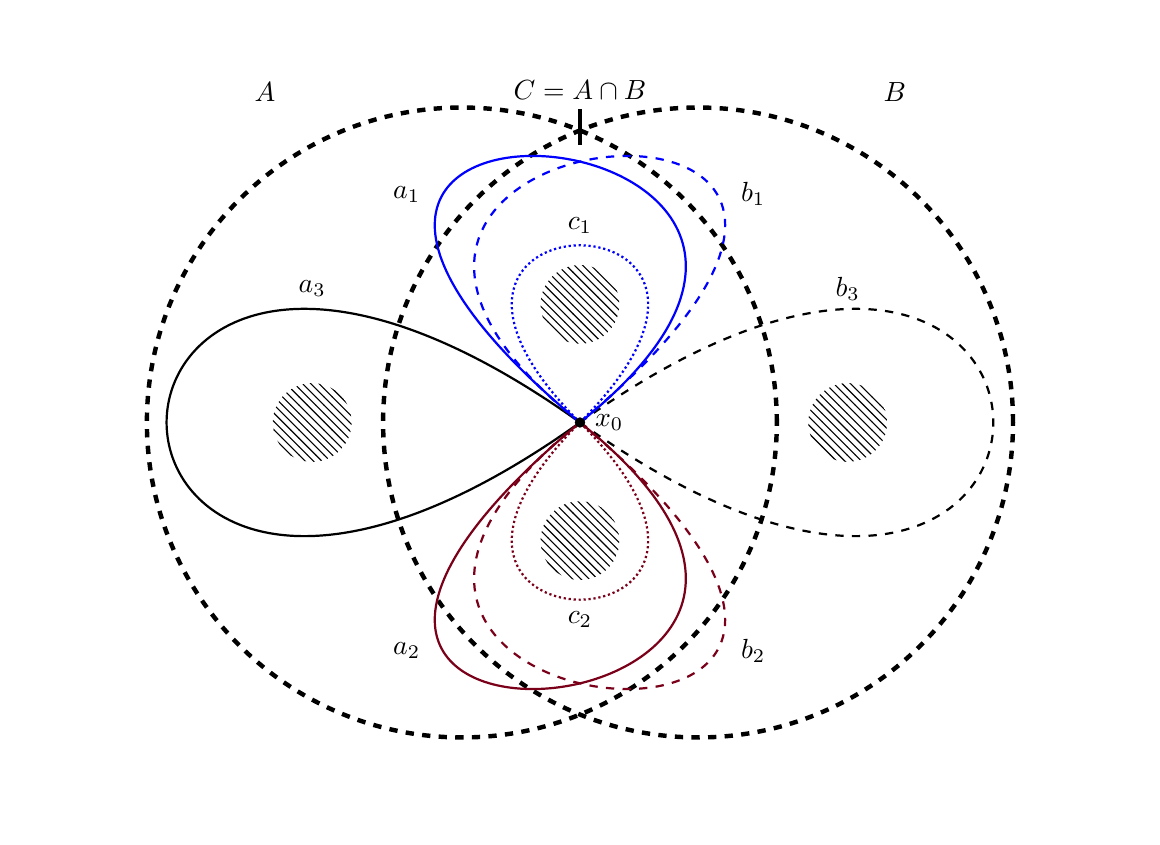
\begin{tikzpicture}
	\draw[ultra thick, dashed] (-1.5,0) circle (4cm);
	\draw[ultra thick, dashed] (1.5,0) circle (4cm);
	\draw[pattern = north west lines, draw=none] (0,1.5) circle (0.5 cm);
	\draw[pattern = north west lines, draw=none] (0,-1.5) circle (0.5 cm);
	\draw[pattern = north west lines, draw=none] (3.4,0) circle (0.5 cm);
	\draw[pattern = north west lines, draw=none] (-3.4,0) circle (0.5 cm);
	
	\draw[thick, color=blue, densely dotted] (0,0) .. controls (-3,3)  and (3,3) ..  (0,0);
	\draw[thick, densely dotted, color=umaroon] (0,0) .. controls (-3,-3)  and (3,-3) ..  (0,0);
	\draw[thick, dashed] (0,0) .. controls (7,5) and (7,-5) .. (0,0);
	\draw[thick] (0,0) .. controls (-7,5) and (-7,-5) .. (0,0);
	
	\draw[thick, color=blue] (0,0) .. controls (-6,5) and (5,4)  .. (0,0);
	\draw[thick, color=blue, dashed] (0,0) .. controls (6,5) and (-5,4)  .. (0,0);
	
	\draw[thick, color=umaroon] (0,0) .. controls (-6,-5) and (5,-4)  .. (0,0);
	\draw[thick, color=umaroon, dashed] (0,0) .. controls (6,-5) and (-5,-4)  .. (0,0);
	
	\node[fill=black, circle, scale = 0.4, label=right:$x_0$] (0,0) {};
	
	\node[] at (-3.4,1.7) {$a_3$};
	\node[] at (3.4,1.7) {$b_3$};
	
	\node[] at (-2.2,2.9) {$a_1$};
	\node[] at (2.2,2.9) {$b_1$};
	
	\node[] at (-2.2,-2.9) {$a_2$};
	\node[] at (2.2,-2.9) {$b_2$};
	
	\node[] at (0,2.5) {$c_1$};
	\node[] at (0,-2.5) {$c_2$};
	
	\node[] at (-4,4.2) {$A$};
	\node[] at (4,4.2) {$B$};
	
	\node[pin={[pin edge={ultra thick,black}]$C=A\cap B$}] at (0,3.4) {};
	%\draw [ultra thick,domain=112:248,samples=400,dashed] plot ({4*cos(\x)+1.5}, {4*sin(\x)});
	
\end{tikzpicture}
\caption{The whole picture of $X$}\label{fig:Xwloops}
\end{figure}
\end{center}


Then letting $x_1$ be the homotopy equivalence class containing $a_1,b_1,c_1$ and $x_2$ be the homotopy class of $a_2, b_2, c_2$, we see

\begin{center}
	\begin{tabular}{l l} \\
		$j_A(i_{AB}(w)) = x_1^9x_2^4x_1^{-4}x_2^3x_1^{-1} $\\
		\\
		$j_B(i_{BA}(w)) = x_1^9x_2^4x_1^{-4}x_2^3x_1^{-1} $\\ \\
	\end{tabular}
\end{center}

So the first thing we would want to do to compute $\pi_1(X)$ from $\pi_1(A), \pi_1(B), \pi_1(C)$ is just consider the free product $\pi_1(A) * \pi_1(B) = \langle a_1,a_2,a_3, b_1, b_2, b_3 \rangle$. Let $w_2 = b_3^4a_1^3b_2^{-1}a_2a_3^4$.
%
Thinking of $w_2$ as tracing the path of loops, we first go around $b_3$ four times, then three times araound $a_1$, then backwards once around $b_2$, forwards once around $a_2$, and then four times around $a_3$.


But wait! Did you catch the problem? Inside of $X$ we went backwards once around $b_2$ and then immediately after that we went forwards once around $a_2$. This is no problem if we are working inside of $A$ or $B$, but when we glue them together to be in $X$, we need $a_2$ and $b_2$ to be the same element. 

Algebraically, the way to do that is to mod out by $a_2b_2^{-1}$ and $b_2a_2^{-1}$ and their inverses - that is, by the group $\langle a_2b_2^{-1}, b_2a_2^{-1} \rangle$.
Supposing we mod out by those two elements, then we see that 
$w_2 = b_3a_1^3 a_3^4$. 

What is the fundamental reason that we modded out by $a_2 b_2^{-1}$? Because $a_2$ and $b_2$ are the same class $x_2$ in $X$. 
Now look at the loop in the intersection $C$ which corresponds to $x_2$. We know it is $c_2$. But what we didn't see in the example of $w_2$ was that $a_1$ and $b_1$ are the same loop in $X$. This corresponds to $c_2$. 

The problem with just taking the free product lies exactly in the intersection. Modding out by $\langle i_{AB}(w) i_{BA}^{-1} (w), i_{BA}(w) i_{AB}^{-1}(w) : w \in \pi_1(C) \rangle$ does a few things. First, it mushes together loops which represent the same loop in the whole space. The mechanism which does that is $i_{AB} i_{BA}^{-1}$. But we can't do that for every pair of loops, so how do we limit which loops contribute to this? Well it has to be loops that are in both $A$ and $B$, which is to say the loops in $C$.

\section{Conclusion}

I think it is easy to get bogged down in notation in understanding the Siefert-van Kampen theorem. I think it becomes a lot clearer with the perspective of following what happens to a given element of $\pi_1(A)*\pi_1(B)$ when you try to think of it as lying in $\pi_1(X)$. Then since the inclusion map is really the only one that makes sense, we should keep track of how each element of $\pi_1(A)$ and $\pi_1(B)$ are included into $\pi_1(X)$. Of course, the issues arise with loops which are \textit{homotopic} to loops in the intersection. For example even though our $a_1$ and $b_1$ were not in $C$, they were homotopic to $c_1$. We use $\pi_1(C)$, or more generally the fundamental group of the intersections to keep track of such loops, and mod out by a relation which forces them to be the same.


\end{document}